\begin{comment}
\end{comment}

\chapter{Simulation de circuits quantiques avec les réseaux de tenseurs}
\label{ann:simulation-circuits-quantiques-avec-reseaux-de-tenseurs}

La simulation classique d'états quantiques est tout sauf évidente. Ces états, appartenant à l'espace d'Hilbert, sont décrit par des vecteurs d'état de taille exponentielle empêchant ainsi leur caractérisation même pour des systèmes de taille modeste. Cette difficulté, présente dans de nombreux domaines tel l'apprentissage-machine, est aussi connue sous le nom de la \textit{malédiction de la dimensionalité}. Cependant, la représentation de certains états physiques intéressants contient parfois de l'information superflue ou une structure inhérente. Par exemple, un état quantique général de $n$ qubits requiert en théorie un vecteur d'état à $2^{n}$ bits, mais un état quantique non-intriqué nécessite seulement $2n$ bits en raison de l'absence de corrélation. Cette idée a alors mené au développement des méthodes de réseaux de tenseurs pour l'étude de système quantique à plusieurs corps en matière condensé dans l'objectif d'obtenir une représentation des états quantiques plus efficace. 

Cette annexe décrit seulement en surface les méthodes de réseaux de tenseur. Pour comprendre les différentes méthodes plus en profondeur, de nombreux tutoriels ont été écrits~\cite{bridgemanHandwavingInterpretiveDance2017,biamonteTensorNetworksNutshell2017,bakerMethodesCalculAvec2021}

%-----------------------------------------------------------------------------%

\section{Réseaux de tenseurs}


Un \textit{tenseur} est un tableau multi-linéaire avec un nombre arbitraire de dimensions encodant une certaine quantité d'information. Plus formellement, un tenseur $T[d_{1}, d_{2}, \dots, d_{m}]$ de rang $m$ avec dimensions $d_{1} \times d_{2} \times \dots \times d_{m}$ est un élément de l'ensemble $\mathbb{C}^{d_{1} \times d_{2} \times \dots \times d_{m}}$. Ceux-ci sont aussi interprétés comme une fonction définie sur un domaine discret. Les tenseurs possèdent une représentation géométrique simple, permettant de visualiser aisément leur caractéristiques principales. Par exemple, un scalaire, un vecteur et une matrice, correspondant respectivement à un tenseur de rang 0, 1 et 2, sont représentés par une forme géométrique avec une patte pour chaque indice tel qu'illustré à la figure~\ref{fig:tensor}.

\begin{figure}[ht!]
    \centering
    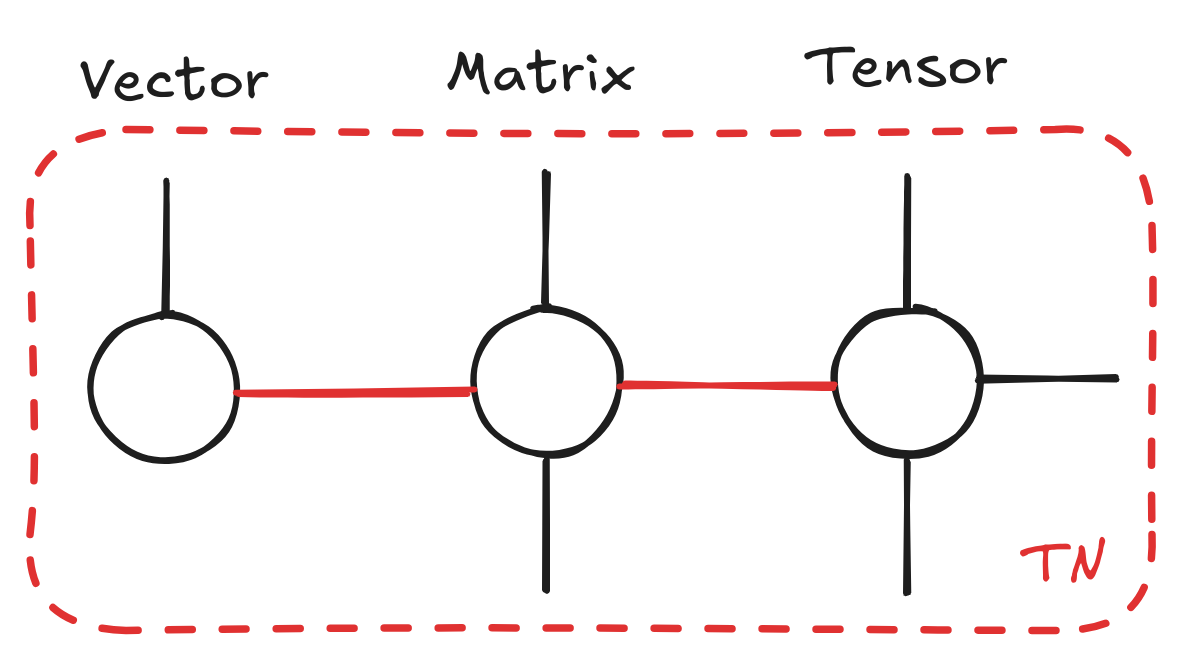
\includegraphics[width=0.6\textwidth]{figures/tensor.png}
    \caption{}
    \label{fig:tensor}
\end{figure}


Plusieurs opérations peuvent être appliquées sur des tenseurs. La contraction de deux tenseurs 

D'autres opérations sont aussi importantes. La trace d'un tenseur est la sommation sur les

D'autres opérations, comme la trace, la décomposition, le regroupement et la séparation.

Les réseaux de tenseurs sont une collection de tenseurs partageant entre eux certains indices.




%-----------------------------------------------------------------------------%

\section{État en produit de matrices et opérateur en produit de matrices}

Un \textit{état en produit de matrices} (« Matrix Product State ») (MPS) est une représentation efficace d'un état quantique.




%-----------------------------------------------------------------------------%

\section{Simulation de circuits quantiques}

\begin{comment}
\subsection*{Plan}

\begin{enumerate}
    \item Décrire le lien entre les circuits quantiques et les réseaux de tenseurs
    \item Décrire les différentes méthodes de simulation (MPS-MPO et réseau de tenseurs général)
    \item Décrire la méthode d'échantillonage
\end{enumerate}

\subsection*{Références}

1. Gray, J. quimb: A python package for quantum information and many-body calculations. Journal of Open Source Software 3, 819 (2018).

2. Ferris, A. J. and Vidal, G. Perfect Sampling with Unitary Tensor Networks. Phys. Rev. B 85, 165146 (2012).
\end{comment}


Afin d'obtenir des échantillons à partir d'un réseau de tenseur, deux méthodes sont possibles. D'abord, une réprésentation dense de la fonction d'onde peut être obtenue en contractant le réseau. Les états sont alors simplement obtenus en pigeant selon la distribution de probabilité trouvée. Une méthode alternative utilise plutôt ~\cite{ferrisPerfectSamplingUnitary2012}. 






%-----------------------------------------------------------------------------%
